\subsubsection{Controller}

\rule{\textwidth}{0.4pt}
\class{CookieController}
\begin{minipage}{0.4\textwidth}
    \begin{figure}[H]
        {\centering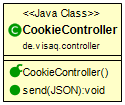
\includegraphics[scale = 0.7]{media/frontend/controller/CookieController_Class.png}}
    \end{figure}
    \end{minipage} \hfill
    \begin{minipage}{0.6\textwidth}
Der CookieController kapselt und übergibt die Cookies dem Server, welcher diese speichert.
\end{minipage}

Methoden: \begin{itemize} 
    \item \emph{public synchronized void send(JSON json)} Das Senden der BEnutzer Daten erfolgt hier, indem diese als JSON Parameter übergeben werden.
\end{itemize}


\rule{\textwidth}{0.4pt}
\class{AngularController}
\begin{minipage}{0.4\textwidth}
    \begin{figure}[H]
        {\centering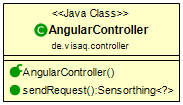
\includegraphics[scale = 0.7]{media/frontend/controller/AngularController_Class.png}}
    \end{figure}
    \end{minipage} \hfill
    \begin{minipage}{0.6\textwidth}
Der AngularController stellt Anfragen an das Backend und wandelt die erhaltenen JSON Dateien in Sensorthings um. Dieser wird mithilfe des jsweet-Angular-4 Candies implementiert und erleichtert so die Kommunikation zwischen backend und frontend.
\end{minipage}
Methoden: \begin{itemize}
    \item \emph{public synchronized Sensorthing<?> sendRequest()} Eine synchrone Anfrage an das Backend auf dem Server welche die gewünschten Daten abfragt und diese dann dem Benutzer anzeigt.
\end{itemize}